%%%%%%%%%%%%%%%%%%%%%%
%%Options for presentations (in-class) and handouts (e.g. print). 
%\documentclass[pdf]{beamer} 
\documentclass[pdf,handout]{beamer}
\usepackage{pgfpages}
\pgfpagesuselayout{2 on 1}[letterpaper,border shrink=5mm]

%%%%%%%%%%%%%%%%%%%%%%
%Change this for different slides so it appears in bar
\usepackage{authoraftertitle}
\date{$\mathbb{R}^n$: Planes}

%%%%%%%%%%%%%%%%%%%%%%
%% Upload common style file
\usepackage{LyryxLinearAlgebraSlidesStyle}

\begin{document}

%%%%%%%%%%%%%%%%%%%%%%%
%% Title Page and Copyright Common to All Slides

%Title Page
\input ../frontmatter/titlepage.tex

%LOTS Page
%\input frontmatter/lyryxopentexts.tex

%Copyright Page
\input ../frontmatter/copyright.tex

%%%%%%%%%%%%%%%%%%%%%%%%%

\section{Equations of Planes}
%-------------- start slide -------------------------------%
\frame{\frametitle{Equations of Planes}
\begin{block}{}
Given a point $P_0$ and a nonzero vector $\vec{n}$, there is
a unique plane containing $P_0$ and orthogonal to $\vec{n}$.

\begin{picture}(2,0.9)
\put(1.5,0.1){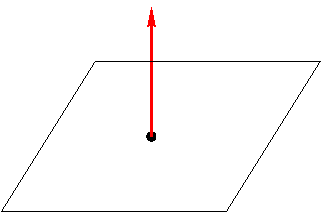
\includegraphics[scale=.6]{../figures/vectors-18a.pdf}}
\put(2.0,0.3){{\footnotesize $P_0$}}
\put(2.15,0.85){{\footnotesize \alert{$\vec{n}$}}}
\end{picture}
\end{block}
\pause
\begin{definition}
A nonzero vector $\vec{n}$ is a \alert{normal vector}
to a plane if and only if $\vec{n}\dotprod\vec{v}=0$ for
every vector $\vec{v}$ in the plane,
i.e., $\vec{n}$ is orthogonal to every vector in the plane.
\end{definition}
}
%-------------- end slide -------------------------------%

%-------------- start slide -------------------------------%
\frame{
\begin{block}{}
Consider a plane containing a point $P_0$ and orthogonal to vector
$\vec{n}$, and let $P$ be an arbitrary point on this plane.
\pause
Then
$\vec{n}\dotprod\overrightarrow{P_0P} = 0$,

\begin{picture}(2,1.0)
\put(1.5,0.1){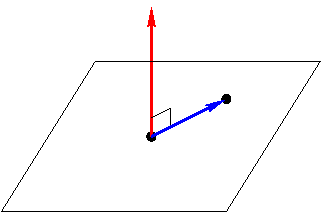
\includegraphics[scale=.6]{../figures/vectors-18b.pdf}}
\put(2.0,0.3){{\footnotesize $P_0$}}
\put(2.15,0.85){{\footnotesize \alert{$\vec{n}$}}}
\put(2.45,0.55){{\footnotesize $P$}}
\end{picture}
\pause

or, equivalently,
\[ \vec{n}\dotprod
(\overrightarrow{0P}-\overrightarrow{0P_0}) = 0,\]
\pause
and is called a \alert{vector equation} of the plane. 
\pause
The vector equation can also be written as
\[ \vec{n}\dotprod \overrightarrow{0P}=
\vec{n}\dotprod\overrightarrow{0P_0}.\]
\end{block}
}
%-------------- end slide -------------------------------%

%-------------- start slide -------------------------------%
\frame{
\begin{block}{}
Suppose a plane contains a fixed point
$P_0=(x_0,y_0,z_0)$ and has normal vector
\[ \vec{n}=\left[\begin{array}{c}
a \\ b \\ c \end{array}\right].\]
\pause
Let $P=(x,y,z)$ denote an arbitrary point on the plane.
\pause
Since 
$\vec{n}\dotprod \overrightarrow{0P}=
\vec{n}\dotprod\overrightarrow{0P_0}$,
\pause
\[ \left[\begin{array}{c}
a \\ b \\ c \end{array}\right]
\dotprod
\left[\begin{array}{c}
x \\ y \\ z \end{array}\right]
=
\left[\begin{array}{c}
a \\ b \\ c \end{array}\right]
\dotprod
\left[\begin{array}{c}
x_0 \\ y_0 \\ z_0 \end{array}\right]. \]
\pause
Thus
\[ ax+by+cz=ax_0+by_0+cz_0,\]
where $d=ax_0+by_0+cz_0$ is simply a scalar.
\pause

A \alert{scalar equation} of the plane has the form
\[ ax+by+cz=d,\mbox{ where }  a,b,c,d\in\RR.\]
\end{block}
}
%-------------- end slide -------------------------------%

%-------------- start slide -------------------------------%
\frame{
\begin{problem}\em
Find an equation of the plane containing $P_0(1, -1, 0)$ and
orthogonal to
$\vec{n} =\left[\begin{array}{ccc}
-3 & 5 & 2 \end{array}\right]^T$.
\end{problem}
\pause
\begin{solution}\em
A \alert{vector equation} of this plane is
\[ \left[\begin{array}{r}
-3 \\ 5 \\ 2 \end{array}\right]
\dotprod
\left[\begin{array}{c}
x-1 \\ y+1 \\ z \end{array}\right] = 0.\]
\pause

Thus, a \alert{scalar equation} of this plane is
\[
-3x+5y+2z=-3(1)+5(-1)+2(0) = -8,\]
i.e., the plane has scalar equation
\[ -3x + 5y +2z=-8.\]
\end{solution}
}
%-------------- end slide -------------------------------%

\section{Shortest distance from a point to a plane}
%-------------- start slide -------------------------------%
\frame{\frametitle{Shortest distance from a point to a plane}
\begin{problem}\em
Find the shortest distance from the point $P=(2,3,0)$ to the plane
with equation $5x+y+z=-1$, and find the point $Q$ on the plane
that is closest to $P$.
\end{problem}
{\alert{(wb example)}}
\pause
\begin{solution}\em

\begin{picture}(2,1.4)
\put(0.2,0.2){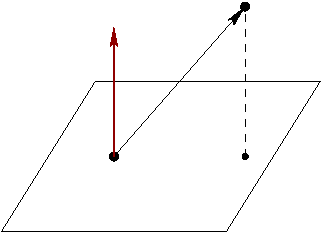
\includegraphics[scale=.7]{../figures/vectors-18.pdf}}
\put(0.6,0.4){\small $P_0$}
\put(0.8,1.0){\small $\vec{n}$}
\put(1.2,0.4){\small $Q$}
\put(1.4,1.2){\small $P=(2,3,0)$}
\pause
\put(2.2,1.0){\small Pick an arbitrary point $P_0$ on the plane.}
\pause
\put(2.2,0.7){\small Then
$\overrightarrow{QP}=\proj_{\vec{n}}\overrightarrow{P_0P}$,}
\pause
\put(2.3,0.5){$\vectlength \overrightarrow{QP}\vectlength$ is the shortest distance,}
\pause
\put(2.3,0.3){and
$\overrightarrow{0Q}=\overrightarrow{0P}-\overrightarrow{QP}$. }
\end{picture}
\pause

$\vec{n}=\left[\begin{array}{c}
5 \\ 1 \\ 1 \end{array}\right]$.
\pause
Choose $P_0=(0,0,-1)$.
\pause
Then $\overrightarrow{P_0P}
= \left[\begin{array}{c}
2 \\ 3 \\ 1 \end{array}\right]$.
\end{solution}
}
%-------------- end slide -------------------------------%

%-------------- start slide -------------------------------%
\frame{
\begin{solution}[continued]\em
\begin{picture}(2,1.1)
\put(0.2,0.0){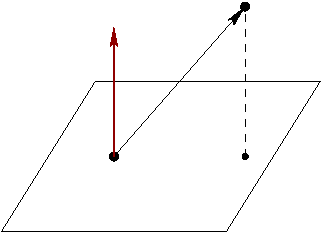
\includegraphics[scale=.7]{../figures/vectors-18.pdf}}
\put(0.6,0.2){\small $P_0$}
\put(0.8,0.8){\small $\vec{n}$}
\put(1.2,0.2){\small $Q$}
\put(1.4,1.0){\small $P=(2,3,0)$}
\put(2.2,0.6){\small $\overrightarrow{P_0P}
= \left[\begin{array}{c}
2 \\ 3 \\ 1 \end{array}\right]$
and
$\vec{n} = \left[\begin{array}{c}
5 \\ 1 \\ 1 \end{array}\right]$.}
\end{picture}
\vspace*{-.2in}

\pause
\[ \overrightarrow{QP}=
\proj_{\vec{n}}\overrightarrow{P_0P}
\pause
= \left( \frac{\overrightarrow{P_0P}\dotprod\vec{n}}
{\vectlength \vec{n}\vectlength ^2} \right) \vec{n}
\pause
=\frac{14}{27}
\left[\begin{array}{c}
5 \\ 1 \\ 1 \end{array}\right]. \]
\pause

Since $\vectlength \overrightarrow{QP}\vectlength= \frac{14}{27}\sqrt{27}
=\frac{14\sqrt{3}}{9}$, 
\pause
the shortest distance from $P$ to the plane is $\frac{14\sqrt{3}}{9}$.
\end{solution}
}
%---------------------end slide--------------------%

%----------------------start slide-------------------%
\frame{
\begin{solution}[continued]\em
To find $Q$, we have
\[ \overrightarrow{0Q} = \overrightarrow{0P} - \overrightarrow{QP}
\pause
= 
\left[\begin{array}{c}
2 \\ 3 \\ 0 \end{array}\right]
-
\frac{14}{27}
\left[\begin{array}{c}
5 \\ 1 \\ 1 \end{array}\right] 
\pause
=  \frac{1}{27}
\left[\begin{array}{c}
-16 \\ 67 \\ -14 \end{array}\right].\]
\pause
Therefore
$Q=\left( -\frac{16}{27}, \frac{67}{27}, -\frac{14}{27}\right)$.
\end{solution}
}
%-------------- end slide -------------------------------%

\section{The Cross Product}


%-------------- start slide -------------------------------%
\frame{\frametitle{The Cross Product}
\begin{definition}
Let $\vec{u}=\left[\begin{array}{ccc}
u_1 & u_2 & u_3 \end{array}\right]^T$
and 
$\vec{v}=\left[\begin{array}{ccc}
v_1 & v_2 & v_3 \end{array}\right]^T$.
Then
\[
\vec{u}\times\vec{v} =
\left[\begin{array}{c}
u_2v_3-u_3v_2 \\
-(u_1v_3-u_3v_1) \\
u_1v_2-u_2v_1
\end{array}\right].\]
\end{definition}

\uncover<2->{
{\bf Note.} 
$\vec{u}\times\vec{v}$ is a vector that is orthogonal to both
$\vec{u}$ and $\vec{v}$.}
\medskip

\uncover<3->{\alert{A helpful way to remember (once we cover determinants):}
\[
\vec{u}\times\vec{v} =
\left|\begin{array}{ccc}
\vec{i} & \vect{j} & \vect{k} \\
u_1 & u_2 & u_3 \\
v_1 & v_2  & v_3 
\end{array}\right|,
\mbox{ where }
\vec{i} = 
\left[\begin{array}{c}
1 \\ 0 \\ 0 \end{array}\right],
\vec{j} = 
\left[\begin{array}{c}
0 \\ 1 \\ 0 \end{array}\right],
\vec{k} = 
\left[\begin{array}{c}
0 \\ 0 \\ 1 \end{array}\right].
\]}
}
%-------------- end slide -------------------------------%

%--------------------start slide--------------------%
\frame{\frametitle{Computing the Cross Product}

\begin{problem}\em
Find $\vect{u} \times \vect{v}$ for $\vect{u} = \left[ \begin{array}{r} 
1 \\ -1 \\ 2 \end{array}\right], \vect{v} = \left[ \begin{array}{r}
3 \\ -2 \\ 1 \end{array} \right]$. 
\end{problem}

\uncover<2->{
\begin{solution}\em
We will use the equation:
\[
\vec{u}\times\vec{v} =
\left[\begin{array}{c}
u_2v_3-u_3v_2 \\
-(u_1v_3-u_3v_1) \\
u_1v_2-u_2v_1
\end{array}\right]
\]
}

\uncover<3->{
Therefore,
\[
\vec{u}\times\vec{v} =
\left[\begin{array}{c}
(-1)(1)-(2)(-2) \\
-((1)(1)-(2)(3)) \\
(1)(-2)-(-1)(3)
\end{array}\right]
 = \left[
\begin{array}{r}
3 \\
5 \\
1
\end{array}
\right]
\]
}
\end{solution}

}
%------------------------end slide----------------------%

%-------------- start slide -------------------------------%
\frame{\frametitle{Properties of the Cross Product}
\begin{theorem}\em
Let $\vec{u}, \vec{v}$ and $\vec{w}$ be in $\RR^3$.
\begin{enumerate}
\item<2->
$\vec{u}\times\vec{v}$ is a vector.
\item<3->
$\vec{u}\times\vec{v}$ is orthogonal to both $\vec{u}$ and $\vec{v}$.
\item<4->
$\vec{u}\times\vec{0}=\vec{0}$ and
$\vec{0}\times\vec{u}=\vec{0}$.
\item<5->
$\vec{u}\times\vec{u}=\vec{0}$.
\item<6->
$\vec{u}\times\vec{v} = - (\vec{v}\times\vec{u})$.
\item<7->
$(k\vec{u})\times\vec{v}
= k(\vec{u}\times\vec{v})
=\vec{u}\times(k\vec{v})$ for any scalar $k$.
\item<8->
$\vec{u}\times(\vec{v} + \vec{w}) =
\vec{u}\times\vec{v} + \vec{u}\times\vec{w}$.
\item<9->
$(\vec{v} + \vec{w})\times\vec{u}=
\vec{v}\times\vec{u} + \vec{w}\times\vec{u}$.
\end{enumerate}
\end{theorem}
}
%-------------- end slide -------------------------------%


%-------------- start slide -------------------------------%
\frame{
\begin{problem}\em
Find all vectors orthogonal to both 
$\vec{u}=\left[\begin{array}{ccc}
-1 & -3 & 2 \end{array}\right]^T$
and
$\vec{v}=\left[\begin{array}{ccc}
0 & 1 & 1 \end{array}\right]^T$.
\end{problem}

\uncover<2->{
\begin{solution}\em
\[
\vec{u}\times\vec{v} =
\left|\begin{array}{crr}
\vec{i} &  -1 & 0 \\
\vec{j} & -3 & 1 \\
\vec{k} & 2 & 1
\end{array}\right|
= -5\vec{i} +\vec{j}-\vec{k}
= \left[\begin{array}{r}
-5 \\ 1 \\ -1 \end{array}\right].
\]}

\uncover<3->{
Any scalar multiple of $\vec{u}\times\vec{v}$ is also
orthogonal to both $\vec{u}$ and $\vec{v}$, so 
\[ t\left[\begin{array}{r}
-5 \\ 1 \\ -1 \end{array}\right], t\in\RR, \]
gives all vectors orthogonal to both $\vec{u}$ and $\vec{v}$.

}
\end{solution}
}
%-------------- end slide -------------------------------%

%-------------- start slide -------------------------------%
\frame{
\begin{problem}\em
Let $A=(1,-1,2)$, $B=(2,0,-1)$ and $C=(0,-2,3)$ be points
in $\RR^3$.  
These points do no all lie on the same line
\alert{(how can you tell?).}
\pause
Find an equation for the plane containing $A$, $B$, and $C$.
\end{problem}
(wb example)
\pause
\begin{solution}\em
\begin{picture}(2,1.1)
\put(0.2,0.1){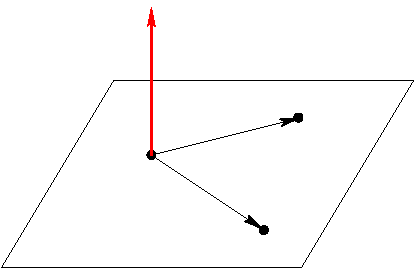
\includegraphics[scale=.6]{../figures/vectors-22.pdf}}
\put(0.65,0.5){\scriptsize{$A$}}
\put(1.3,0.2){\scriptsize{$B$}}
\put(1.45,0.65){\scriptsize{$C$}}
\pause
\put(2.1,0.7){\footnotesize{$\overrightarrow{AB}$ and $\overrightarrow{AC}$
lie in the plane, \pause so}}
\put(2.2,0.5){\footnotesize{$\vec{n}=
\overrightarrow{AB}\times\overrightarrow{AC}$ is a normal to the plane.}}
\put(0.85,0.95){\scriptsize\alert{$\vec{n}$}}
\pause
\put(1.9,.1){\footnotesize
$\overrightarrow{AB}=
\left[\begin{array}{r} 1 \\ 1 \\ -3 \end{array}\right],~
\pause
\overrightarrow{AC}=
\left[\begin{array}{r} -1 \\ -1 \\ 1 \end{array}\right]$,
\pause
and
$\vec{n}=
\left[\begin{array}{r} -2 \\ 2 \\ 0 \end{array}\right]$.}
\end{picture}
\pause

\[
\mbox{Therefore} \;
 -2x + 2y =
\left[\begin{array}{r} -2 \\ 2 \\ 0 \end{array}\right]
\bullet
\left[\begin{array}{r} 0 \\ -2 \\ 3 \end{array}\right]
\pause
= -4 \]
i.e. $-2x + 2y = -4$ is an equation of the plane. 
\end{solution}
}
%-------------- end slide -------------------------------%
%-------------- start slide -------------------------------%
\frame{\frametitle{Lecture Part II}
	
}
%----------------------end slide----------------%


%-------------- start slide -------------------------------%
\frame{\frametitle{Distance between Skew Lines}
\begin{problem}\em
Given two lines
\[ 
L_1:
\left[\begin{array}{c}
x \\ y \\ z \end{array}\right]
=
\left[\begin{array}{r}
3 \\ 1 \\ -1 \end{array}\right]
+
s\left[\begin{array}{r}
1 \\ 1 \\ -1 \end{array}\right]
\mbox{ and }
L_2:
\left[\begin{array}{c}
x \\ y \\ z \end{array}\right]
=
\left[\begin{array}{r}
1 \\ 2 \\ 0 \end{array}\right]
+ 
t\left[\begin{array}{r}
1 \\ 0 \\ 2 \end{array}\right],
\]
\vspace*{-.15in}
\begin{itemize}
\item[A.]
Find the shortest distance between $L_1$ and $L_2$.
\item[B.]
Find the shortest distance between $L_1$ and $L_2$, \alert{and} 
find the points $P$ on $L_1$ and $Q$ on $L_2$ that are closest
together.
\end{itemize}
\end{problem}

}
%----------------------end slide----------------%


%---------------------start slide-------------%
\frame{\frametitle{Solution A}

\begin{solution}\em

\begin{picture}(2,1.3)
\put(0.2,0.2){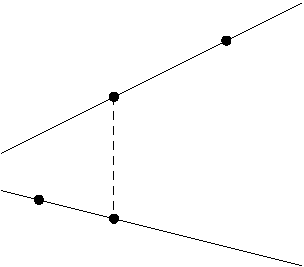
\includegraphics[scale=.6]{../figures/vectors-19.pdf}}
\put(0.25,0.3){\scriptsize $P_2$}
\put(0.6,0.25){\scriptsize $Q$}
\put(0.6,0.95){\scriptsize $P$}
\put(1.07,0.9){\scriptsize $P_1$}
\put(1.6,1){\scriptsize Choose $P_1(3,1,-1)$ on $L_1$ and
$P_2(1,2,0)$ on $L_2$.}
\put(1.6,0.6){\scriptsize 
Let $\vec{d}_1=
\left[\begin{array}{r}
1 \\ 1 \\ -1 \end{array}\right]$ 
and $\vec{d}_2=
\left[\begin{array}{r}
1 \\ 0 \\ 2 \end{array}\right]$ denote direction vectors}
\put(1.65,0.35){\scriptsize for $L_1$ and $L_2$, respectively.}
\end{picture}

\end{solution}
}
%-------------- end slide -------------------------------%

%-------------- start slide -------------------------------%
\frame{
\begin{solution}[continued]\em

\begin{picture}(2,1.3)
\put(0.2,0.2){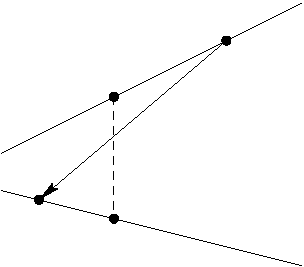
\includegraphics[scale=.6]{../figures/vectors-20.pdf}}
\put(0.05,0.3){\scriptsize $P_2(1,2,0)$}
\put(0.6,0.25){\scriptsize $Q$}
\put(0.6,0.95){\scriptsize $P$}
\put(1.07,0.95){\scriptsize $P_1(3,1,-1)$}
\put(2.0,0.8){\scriptsize $\vec{d}_1=
\left[\begin{array}{r}
1 \\ 1 \\ -1 \end{array}\right]$,
$\vec{d}_2=
\left[\begin{array}{r}
1 \\ 0 \\ 2 \end{array}\right]$}
\put(2.0,0.4){\scriptsize The shortest distance between
$L_1$ and $L_2$ is the length}
\put(2.05,0.25){\scriptsize of the projection of 
$\overrightarrow{P_1P_2}$ onto
$\vec{n}=\vec{d}_1\times\vec{d}_2$.}
\end{picture}


\uncover<2->{

\[ 
\overrightarrow{P_1P_2}=
\left[\begin{array}{r}
-2 \\ 1 \\ 1 \end{array}\right]
\mbox{ and }
\vec{n}=
\left[\begin{array}{r}
1 \\ 1 \\ -1 \end{array}\right]
\times
\left[\begin{array}{r}
1 \\ 0 \\ 2 \end{array}\right]
=
\left[\begin{array}{r}
2 \\ -3 \\ -1 \end{array}\right]
\]}

\uncover<3->{

\[ \proj_{\vec{n}}\overrightarrow{P_1P_2}
=
\left( \frac{\overrightarrow{P_1P_2}\dotprod\vec{n}}{\vectlength \vec{n} \vectlength^2} \right) \vec{n},
\mbox{ and }
\vectlength \proj_{\vec{n}}\overrightarrow{P_1P_2} \vectlength 
=
\frac{|\overrightarrow{P_1P_2}\dotprod\vec{n}|}{\vectlength \vec{n} \vectlength}.
\]}

\uncover<4->{
Therefore, the shortest distance between $L_1$ and $L_2$ is
$\frac{|-8|}{\sqrt{14}}=\frac{4}{7}\sqrt{14}$.}
\end{solution}
}
%-------------- end slide -------------------------------%

%-------------- start slide -------------------------------%
\frame{\frametitle{Solution B}

\begin{solution}\em

\begin{picture}(2,1.3)
\put(0.2,0.2){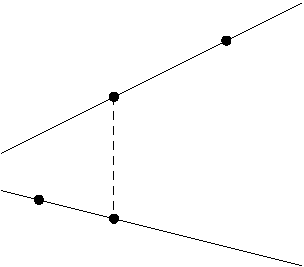
\includegraphics[scale=.6]{../figures/vectors-19.pdf}}
\put(0.05,0.3){\scriptsize $P_2(1,2,0)$}
\put(0.6,0.25){\scriptsize $Q$}
\put(0.6,0.95){\scriptsize $P$}
\put(1.07,0.95){\scriptsize $P_1(3,1,-1)$}
\put(2.0,1.2){\scriptsize
$\vec{d}_1=
\left[\begin{array}{r}
1 \\ 1 \\ -1 \end{array}\right]$,
$\vec{d}_2=
\left[\begin{array}{c}
1 \\ 0 \\ 2 \end{array}\right]$;}
\put(2.0,0.7){\scriptsize
$\overrightarrow{0P}=
\left[\begin{array}{c}
3+s \\ 1 + s \\ -1 -s \end{array}\right]$
for some $s\in\RR$;} 
\put(2.0,0.2){\scriptsize
$\overrightarrow{0Q}=
\left[\begin{array}{c}
1+t \\ 2  \\ 2t \end{array}\right]$
for some $t\in\RR$.}
\end{picture}

\uncover<2->{
Now $\overrightarrow{PQ}=\left[\begin{array}{ccc}
-2-s+t & 1-s & 1+s+2t \end{array}\right]^T$ is orthogonal
to both $L_1$ and $L_2$, so 
\[ \overrightarrow{PQ}\dotprod\vec{d}_1 = 0
\mbox{ and }
\overrightarrow{PQ}\dotprod\vec{d}_2 = 0,\]}
\uncover<3->{i.e., 
\vspace*{-.3in}
\begin{eqnarray*}
-2-3s-t &= & 0 \\
s + 5t & = & 0.
\end{eqnarray*}}
\vspace*{-.2in}
\end{solution}
}
%----------------------end slide----------------------------%

%------------------start slide---------------------------%
\frame{\frametitle{Solution B}

\begin{solution}[continued]\em
This system has unique solution $s=-\frac{5}{7}$
and $t=\frac{1}{7}$.

\uncover<2->{Therefore,
\vspace*{-.1in}
\[ P=\left(\frac{16}{7}, \frac{2}{7}, -\frac{2}{7}\right)
\mbox{ and }
Q=\left(\frac{8}{7}, 2, \frac{2}{7}\right).\]
\vspace*{-.15in}
}

\uncover<3->{
The shortest distance between $L_1$ and $L_2$ is
$\vectlength \overrightarrow{PQ} \vectlength$.
Since 
\[ P=\left(\frac{16}{7}, \frac{2}{7}, -\frac{2}{7}\right)
\mbox{ and }
Q=\left(\frac{8}{7}, 2, \frac{2}{7}\right),\]
}

\uncover<4->{
\[ \overrightarrow{PQ}
=
\frac{1}{7}\left[\begin{array}{r}
8 \\ 14 \\ 2 \end{array}\right]
-
\frac{1}{7}\left[\begin{array}{r}
16 \\ 2 \\ -2 \end{array}\right]
=
\frac{1}{7}\left[\begin{array}{r}
-8 \\ 12 \\ 4 \end{array}\right],
\]}
\end{solution}
}
%--------------------end slide----------------------%

%--------------------start slide-----------------%
\frame{\frametitle{Solution B}

\begin{solution}[continued]\em
\[
\overrightarrow{PQ}
=
\frac{1}{7}\left[\begin{array}{r}
-8 \\ 12 \\ 4 \end{array}\right]
\]

\uncover<2->{
Therefore
\[ \vectlength \overrightarrow{PQ} \vectlength=
\frac{1}{7}\sqrt{224}=\frac{4}{7}\sqrt{14}.\]
}

\uncover<3->{
The shortest distance between $L_1$ and $L_2$
is $\frac{4}{7}\sqrt{14}$.}
\end{solution}
}

%---------------end slide------------------------------%

%-------------- start slide -------------------------------%
\frame{\frametitle{Area and Volume}
\begin{block}{The Lagrange Identity}
If $\vec{u}, \vec{v}\in\RR^3$, then
\[ \|\vec{u}\times\vec{v}\|^2 =
\|\vec{u}\|^2 \|\vec{v}\|^2 - (\vec{u}\bullet\vec{v})^2.\]
\end{block}
\pause
\begin{proof}
Write
$\vec{u} = \left[\begin{array}{c}
x_1 \\ y_1 \\ z_1 \end{array}\right]$ and
$\vec{v} = \left[\begin{array}{c}
x_2 \\ y_2 \\ z_2 \end{array}\right]$, and work out all the
terms.
\end{proof}
}
%-------------- end slide -------------------------------%

%-------------- start slide -------------------------------%
\frame{
\begin{block}{The length of the cross product}
{\small
As a consequence of the Lagrange Identity and the fact that
\[ \vec{u}\bullet\vec{v} =
\|\vec{u}\|~\|\vec{v}\|\cos\theta,\]
\pause
we have
\vspace*{-.1in}
\begin{eqnarray*}
\|\vec{u}\times\vec{v}\|^2 & = &
\|\vec{u}\|^2 \|\vec{v}\|^2 - (\vec{u}\bullet\vec{v})^2 \\
\pause
& = &
\|\vec{u}\|^2 \|\vec{v}\|^2 -
\|\vec{u}\|^2 \|\vec{v}\|^2 \cos^2\theta \\
\pause
& = &
\|\vec{u}\|^2 \|\vec{v}\|^2(1- \cos^2\theta) \\
\pause
& = & \|\vec{u}\|^2 \|\vec{v}\|^2 \sin^2\theta.
\end{eqnarray*}
\pause
Taking square roots on both sides yields,
\[ \|\vec{u}\times\vec{v}\| = \|\vec{u}\|\|\vec{v}\| \sin\theta.\]
\vspace*{-.1in}
\pause

Note that since $0\leq\theta\leq \pi$, $\sin\theta\geq 0$.
\bigskip
\pause

If $\theta=0$ or $\theta=\pi$, then
$\sin\theta=0$, and $\|\vec{u}\times\vec{v}\|=0$.
\pause
This is consistent with our earlier observation that if
$\vec{u}$ and $\vec{v}$
are parallel, then $\vec{u}\times\vec{v}=\vec{0}$.
}
\end{block}
}
%-------------- end slide -------------------------------%

%-------------- start slide -------------------------------%
\frame{\frametitle{Area of a Parallelogram}
\begin{theorem}\em
Let $\vec{u}$ and $\vec{v}$ be nonzero vectors in $\RR^3$ with
included angle $\theta$.
\pause
\begin{enumerate}
\item
$\|\vec{u}\times\vec{v}\| = \|\vec{u}\|\|\vec{v}\|\sin\theta$,
and is the area of the parallelogram defined by $\vec{u}$ and
$\vec{v}$.
\pause
\item
$\vec{u}$ and $\vec{v}$ are parallel if and only if
$\vec{u}\times\vec{v}=\vec{0}$.
\end{enumerate}
\end{theorem}
\pause
\begin{proof}[Proof of area of parallelogram]
The area of the parallelogram defined by $\vec{u}$ and $\vec{v}$
is $\|\vec{u}\|h$, where $h$ is the height of the parallelogram.

\begin{picture}(3,0.6)
\put(1.6,0.1){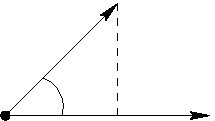
\includegraphics[scale=.6]{../figures/vectors-21.pdf}}
\put(1.8,0.4){\scriptsize $\vec{v}$}
\put(1.9,0.0){\scriptsize $\vec{u}$}
\put(1.75,0.15){\scriptsize $\theta$}
\put(2.1,0.3){\scriptsize $h$}
\end{picture}
\pause
\medskip

$\sin\theta =\frac{h}{\|\vec{v}\|}$, implying that
$h=\|\vec{v}\|\sin\theta$.
\pause
Therefore, the area is 
\vspace*{-.1in}

\[ \|\vec{u}\|\|\vec{v}\|\sin\theta.\] 
\vspace*{-.3in}

\end{proof}
}
%-------------- end slide -------------------------------%

%-------------- start slide -------------------------------%
\frame{\frametitle{Area of a Triangle}
\begin{problem}\em
Find the area of the triangle having vertices
$A(3,-1,2)$, $B(1,1,0)$ and $C(1,2,-1)$.
\end{problem}
\medskip

\uncover<2->{
\begin{solution}\em
The area of the triangle is half the area of the parallelogram
defined by $\overrightarrow{AB}$ and $\overrightarrow{AC}$.}

\uncover<3->{
$\overrightarrow{AB}=
\left[\begin{array}{r}
-2 \\ 2 \\ -2 \end{array}\right]$ and
$\overrightarrow{AC}=
\left[\begin{array}{r}
-2 \\ 3 \\ -3 \end{array}\right]$.}
\uncover<4->{Therefore
\[ \overrightarrow{AB}\times\overrightarrow{AC} =
\left[\begin{array}{r}
0 \\ -2 \\ -2 \end{array}\right],\]}
\uncover<5->{
so the area of the triangle is
$\frac{1}{2} \vectlength \overrightarrow{AB}
\times\overrightarrow{AC} \vectlength = \sqrt{2}$.}
\end{solution}
}
%-------------- end slide -------------------------------%



\section{The Box Product}

%-------------- start slide -------------------------------%
\frame{\frametitle{The Box Product}
\small{
Let 
$\vec{u} = \left[\begin{array}{c}
u_1 \\ u_2 \\ u_3 \end{array}\right]$,
$\vec{v} = \left[\begin{array}{c}
v_1 \\ v_2 \\ v_3 \end{array}\right]$, and
$\vec{w} = \left[\begin{array}{c}
w_1 \\ w_2 \\ w_3 \end{array}\right]$.
\uncover<2->{
Then
\begin{eqnarray*}
\vec{u}\dotprod(\vec{v}\times\vec{w}) & = &
\left[\begin{array}{c}
u_1 \\ u_2 \\ u_3 \end{array}\right] \dotprod
\left[\begin{array}{c}
v_2w_3-v_3w_2 \\ -(v_1w_3-v_3w_1) \\ v_1w_2-v_2w_1 \end{array}\right]\\
& = &
u_1(v_2w_3-v_3w_2) -u_2(v_1w_3-v_3w_1) + u_3(v_1w_2-v_2w_1) \\
& = & 
u_1 \left|\begin{array}{cc}
v_2 & w_2 \\ v_3 & w_3 \end{array}\right| 
-
u_2 \left|\begin{array}{cc}
v_1 & w_1 \\ v_3 & w_3 \end{array}\right| 
+
u_3 \left|\begin{array}{cc}
v_1 & w_1 \\ v_2 & w_2 \end{array}\right| \\
& = & 
\left|\begin{array}{ccc}
u_1 & v_1 & w_1 \\
u_2 & v_2 & w_2 \\
u_3 & v_3 & w_3 \end{array}\right|.
\end{eqnarray*}
}
}


}
%-------------- end slide -------------------------------%

%-------------- start slide -------------------------------%
\frame{\frametitle{The Box Product}

\begin{theorem}\em
If $\vec{u} = \left[\begin{array}{c}
u_1 \\ u_2 \\ u_3 \end{array}\right]$,
$\vec{v} = \left[\begin{array}{c}
v_1 \\ v_2 \\ v_3 \end{array}\right]$, and
$\vec{w} = \left[\begin{array}{c}
w_1 \\ w_2 \\ w_3 \end{array}\right]$.
Then \alert{the box product} is
\[ \vec{u}\dotprod(\vec{v}\times\vec{w})  = 
\det\left[\begin{array}{ccc}
u_1 & v_1 & w_1 \\
u_2 & v_2 & w_2 \\
u_3 & v_3 & w_3 \end{array}\right].
\]
\end{theorem}

\uncover<2->{
{\bf Shorthand:} 
$\vec{u}\dotprod(\vec{v}\times\vec{w}) = \det
\left[\begin{array}{ccc}
\vec{u} & \vec{v} & \vec{w} \end{array}\right]$.}

\uncover<3->{

\begin{theorem}\em
The order of the box product is defined as follows:
\[(\vect{u} \times \vect{v}) \dotprod \vect{w} = \vect{u} \dotprod (\vect{v} \times \vect{w}).\]
\end{theorem}
}
}
%-------------- end slide -------------------------------%



%-------------- start slide -------------------------------%
\frame{\frametitle{The Volume of a Parallelepiped}
\begin{theorem}\em
The volume of the parallelepiped determined by the three
vectors $\vec{u}$, $\vec{v}$, and $\vec{w}$ in $\RR^3$ is
\[ |\vec{u}\dotprod(\vec{v}\times\vec{w})|.\]
\end{theorem}

\uncover<2->{
\begin{problem}\em
Find the volume of the parallelepiped determined by the vectors
$\vec{u}= \left[\begin{array}{r}
2 \\ 1 \\ -1 \end{array}\right]$,
$\vec{v}= \left[\begin{array}{r}
1 \\ 0 \\ 2 \end{array}\right]$,
and
$\vec{w}= \left[\begin{array}{r}
2 \\ 1 \\ 1 \end{array}\right]$.
\end{problem}
}
}
%-------------------end slide------------------%

%--------------------start slide------------------%
\frame{
\begin{solution}\em
The volume of the parallelepiped is $|\vec{u}\bullet(\vec{v}\times\vec{w})|$. 

\pause
Since
$\vec{u}\bullet(\vec{v}\times\vec{w})=
\det \left[\begin{array}{ccc}
\vec{u} & \vec{v} & \vec{w} \end{array}\right]$,
\pause
and
\[
\det\left[ \begin{array}{rrr} 2 & 1 & 2 \\
1 & 0 & 1 \\
-1 & 2 & 1 
\end{array}\right]
\pause
=-2, \]
the volume of the parallelepiped is $|-2|=2$ cubic units.
\end{solution}

}
%-------------- end slide -------------------------------%


\end{document}
